 \documentclass [12pt]{article} 

\usepackage {amsmath}
\usepackage {amsthm}
\usepackage {amssymb}
\usepackage {graphicx} 
\usepackage {float}
\usepackage {multirow}
\usepackage {xcolor}
\usepackage {algorithmic}
\usepackage [ruled,vlined,commentsnumbered,titlenotnumbered]{algorithm2e} \usepackage {array} 
\usepackage {booktabs} 
\usepackage {url} 
\usepackage {parskip} 
\usepackage [margin=1in]{geometry} 
\usepackage [T1]{fontenc} 
\usepackage {cmbright} 
\usepackage [many]{tcolorbox} 
\usepackage [colorlinks = true,
            linkcolor = blue,
            urlcolor  = blue,
            citecolor = blue,
            anchorcolor = blue]{hyperref} 
\usepackage {enumitem} 
\usepackage {xparse} 
\usepackage {verbatim}
\usepackage{listings}
\usepackage{xcolor}
\lstset { %
    language=C++,
    backgroundcolor=\color{black!5}, % set backgroundcolor
    basicstyle=\footnotesize,% basic font setting
}
\newtheorem{theorem}{Theorem}
\newtheorem{remark}{Remark}



\DeclareTColorBox {Solution}{}{breakable, title={Solution}} \DeclareTColorBox {Solution*}{}{breakable, title={Solution (provided)}} \DeclareTColorBox {Instruction}{}{boxrule=0pt, boxsep=0pt, left=0.5em, right=0.5em, top=0.5em, bottom=0.5em, arc=0pt, toprule=1pt, bottomrule=1pt} \DeclareDocumentCommand {\Expecting }{+m}{\textbf {[We are expecting:} #1\textbf {]}} \DeclareDocumentCommand {\Points }{m}{\textbf {(#1 pt.)}} 

\begin {document} 

\vspace {1em} 
\begin {Instruction} 
Adapted From Virginia Williams' lecture notes.
\end {Instruction}  

{\LARGE \textbf {COMP 285 (NC A\&T, Spr `22)}\hfill \textbf {Lecture 13} } 

\begin{centering}
\section*{Hashing}
\end{centering}

\section{Hash tables}
A hash table is a commonly used data structure to store an unordered set of items, allowing constant time inserts, lookups and deletes (in expectation). Every item consists of a unique identifier called a key and a piece of information. For example, the key might be a Social Security Number, a driver's license number, or an employee ID number. The way in which a hash table stores a item depends only on its key, so we will only focus on the key here, but keep in mind that each key is usually associated with additional information that is also stored in the hash table.

A hash table supports the following operations:
\begin{itemize}
  \item Insert($k$): Insert key $k$ into the hash table.
  \item Lookup($k$): Check if key $k$ is present in the table.
  \item Delete($k$): Delete the key $k$ from the table.
\end{itemize}
Each operation will take constant time (in expectation).

\subsection{Implementation}
Let $U$ be the universe of all keys. For example, $U$ could be the set of all 64 bit strings. In this case $|U| = 2^64$. This is a very large universe, but we do not need to store all of these $2^64$ keys, we only need to store a subset $S \subset U$. Suppose that we know that the size of the subset we will need to store is less than or equal to $n$, which is much less than the size of the universe $|U|$. In a hash table of size $n$, each key  $k \in U$ is mapped to one of n ``buckets'' by a hash function $h : U \to \{1, 2, \cdots , n\}$. Since the universe $U$ is much larger than $n$, multiple
keys could map to the same hash bucket. To accommodate this, each bucket contains a linked list of keys currently stored in that bucket.

\textbf{Example}

Suppose we have a hash table of size $n = 5$ with hash function $h(x) = 13x + 2 \mod 5$. After inserting the elements $\{1, 2, 4, 7, 8\}$ the hash table looks like this:

\begin{center}
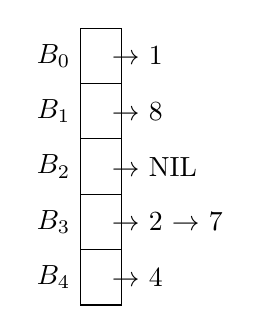
\begin{tikzpicture}
\coordinate (0);
\foreach \t[count=\i from 0,evaluate=\i as\j using int(\i+1)] in {
  1  ,
  8  ,
  NIL  ,
  2 $\rightarrow$ 7,
  4
}
\node at(\i.south)[anchor=north,draw,minimum height=2em,minimum width=1.5em,outer sep=0pt](\j){}
    node at(\j.west)[align=right,left]{$B_{\i}$} 
    node at(\j.east)[align=left,right,xshift=-.7em]{$\rightarrow$ \t};
\end{tikzpicture}
\end{center}

Where arrows denote pointers in the linked lists, and $B_2$ is empty. For example, $1$ is placed into bucket $B_0$ because $h(1) = 15 mod 5 = 0$.

\textbf{Time Complexity} 
ith this setup, the time required to perform an Insert, Lookup, or Delete operation on key $k$ is linear in the length of the linked list for the bucket that key $k$ maps to. We just use the hash function to find the correct bucket for an input key k, and then search the corresponding linked list for the element, inserting or deleting if necessary. Note that an Insert could be performed in constant time by always inserting at the head of the list, but we first need to check if key $k$ is already present.

\textbf{Choice of size of hash table} 
The hash table size is usually chosen so that the size of the hash table is at least as large as the maximum number of keys we will need to store at any point of time. If this condition is violated and the number of keys stored grows much larger than the size of the hash table, an implementation will usually increase the size of the table, and recompute the new table from scratch by mapping all keys to the bigger table. Our analysis ignores these complications and assumes that the number of keys is at most the hash table size.

\textbf{Potential problem with this implementation} 
In order for the operations to be implemented efficiently, we would like the keys to be distributed uniformly amongst the buckets in the hash table. We might hope that all buckets have at most a constant number of keys mapped to them, so that all operations could be performed in constant time. But for any fixed choice hash function $h$, one can always produce a subset of keys $S$ such that all keys in $S$ are mapped to the same location in the hash table. In this case, the running times of all operations will be linear in the number of keys - far from the constant we were hoping for. Thus, for a fixed hash function $h$, it is impossible to give worst case guarantees for the running times of hash table operations.

\textbf{Possible Solutions} 
There are two styles of analysis that we could use to circumvent this problem: 

\begin{enumerate}
  \item Assume that the set of keys stored in the hash table is random, or 
  \item Assume that the hash function $h$ is random. 
\end{enumerate}

Both are plausible alternatives. The problem with the first alternative is that it is hard to justify that the set of keys stored in the hash table is truly random. It would be more satisfying to have an analysis that works for any subset of keys currently in the hash table. In these notes, we will explore the second alternative, i.e., assume that the hash function $h$ is random.

\section{Hashing with a completely random hash function}

What does it mean for $h$ to be random? One possibility is that $h$ is chosen uniformly and at random from amongst the set of all hash functions $h : U → \{1, 2, \cdots , n\}$. In fact picking such a hash function is not really practical. Note that there are $n^{|U|}$ possible hash functions. Representing just one of these hash functions requires $\log ( n^{|U|} ) = |U|\log n$ bits. In fact, this means we need to write down $h(x)$ for every $x \in U$ in order to represent $h$. That's a lot of storage space! Much more than the size of the set we are trying to store in the hash table. One could optimize this somewhat by only recording $h(x)$ for all keys $x$ seen so far (and generating $h(x)$ randomly on the fly when a new $x$ is encountered), but this is impractical too. How would we check if a particular key $x$ has already been encountered? Looks like we would need a hash table for that. But wait, isn't that what we set out to implement? Overall, it is clear that picking a completely random hash function is completely impractical.

Despite this, we will analyze hashing assuming that we have a completely random hash function and then explain how this assumption can be replaced by something that is practical.

\textbf{Expected cost of hash table operations with random hash functions} 

What is the expected cost of performing any of the operations Insert, Lookup, or Delete with a random hash function? Suppose that the keys currently in the hash table are $x_1, \cdots, x_n$. Consider an operation involving key $x_i$ . The cost of the operation is linear in the size of the hash bucket that $x_i$ maps to. Let $X$ be the size of the hash bucket that $x_i$ maps to. $X$ is a random variable and

\begin{align*}
  \mathbb{E}[X] &= \sum_{j=1}^n \mathbb{P}[h(x_i) = h(x_j)] \\
  &= 1 + \sum_{j\neq i} \mathbb{P}[h(x_i) = h(x_j)] \tag{We are guaranteed to collide with ourselves} \\
  &= 1 + \frac{n-1}{n} \leq 2
\end{align*}
Here the last step follows from the fact that $\mathbb{P}[h(x_i ) = h(x_j )] = 1/n$ when $h$ is random. Note that each key appears in the hash table at most once.

Thus the expected cost of any hashing operation is a constant.

\subsection{Universal Hash Functions}
Can we retain the expected cost guarantee of the previous section with a much simpler (i.e.,practical) family of hash functions? In the analysis of the previous section, the only fact we used about random hash functions was that $\mathbb{P}[h(x_i ) = h(x_j )] = 1/n$. Is it possible toconstruct a small, practical subset of hash functions with this property?

Thinking along these lines, in 1978, Carter and Wegman introduced the notion of universal hashing: Consider a family $F$ of hash functions from $U to \{1, 2, \cdots , n\}$. We say that $F$ isuniversal if, for every $x_i \neq x_j$, for an $h$ chosen randomly from $F$ , $\mathbb{P}[h(xi ) = h(xj )] \leq 1/n$.

Clearly the analysis of the previous section shows that for any universal family, the constant expected running time guarantee applies. The family of all hash functions is universal. Is there a simpler universal family?

\section{A universal family of hash functions} 
Suppose that the elements of the $U$ are encoded as non-negative integers in the range ${0, \cdots, |U| - 1}$. Pick a prime $p \geq |U|$. For $a, b \in \{0, \cdots p - 1\}$, consider the family of hash functions 

$$
h_{a,b}(x) = (ax + b \mod p) \mod n
$$

where $a \in \{1, \cdots , p - 1\}$ and $b \in {0, 1, \cdots , p - 1}$. 

\textbf{Proposition 1}. \textit{This family of hash functions $F$ is universal}. 

In order to prove this statement, first, let’s count the number of hash functions in this family $F$ . We have $p-1$ choices for $a$, and $p$ choices for $b$, so $|F| = p(p-1)$. In order to prove that $F$ is universal, we need to show that for an $h$ chosen randomly from $F$ , $\mathbb{P}[h(x_i ) = h(x_j )] \leq 1/n$. Since there are $p(p - 1)$ hash functions in $F$ , this is equivalent to showing that the number of hash functions in $F$ that map $x_i$ and $x_j$ to the same output is less than or equal to $\frac{p(p-1)}{n}$ . To show that this is true, first consider how $h_{a,b}$ behaves without the $\mod n$. Call these functions $f_{a,b}$:
$$
f_{a,b}(x) = ax + b \mod p 
$$
The $f_{a,b}$ have the following useful property: 

\textbf{Proposition 2.} \textit{For a given $x_1, x_2, y_1, y_2 \in \{0, \cdots , p - 1\}$ such that $x_1 \neq x_2$ there exists only one function $f_{a,b}$ such that $f_{a,b}(x_1) = y_1$, and $f_{a,b}(x_2) = y_2$}

 Proof. Solve the above two equations for $a$ and $b$:

 \begin{align*}
  ax_1 + b &\equiv y_1 (\mod p) \\
  ax_2 + b &\equiv y_2 (\mod p)
\end{align*}
By subtracting the two equations, we get:
$$
a(x_1 - x_2) \equiv y_1 - y_2 (\mod 6)
$$
Since $p$ is prime and $x1 \neq x2$, the above equation has only one solution for $a \in \{0, \cdots , p -1\}$.
Then
$$
b \equiv y_1 - ax_1 (\mod p)
$$
So we have found the unique a and b such that $f_{a,b}(x_1) = y_1$ and $f_{a,b}(x_2) = y_2.$

In the above proof, note that $a = 0$ only when $y_1 = y_2 = b$. This is why we restrict $a \neq 0$, we don’t want the hash function mapping all elements to the same value $b$. Now, we have shown that for a given $x_1, x_2$, for each selection of $y_1, y_2$ with $y_1 \neq y_2$, there is exactly one function $f_{a,b}$ that maps $x_1$ to $y_1$ and $x_2$ to $y_2$. So, in order to find out how many functions $h_{a,b}$ map $x_1$ and $x_2$ to the same value $\mod n$, we just need to count the number of pairs $(y_1, y_2)$ where $y_1 \neq y_2$ and $y_1 \equiv y_2 (mod n)$. There are $p$ possible selections of $y_1$ for this pair, and then $\leq (p - 1)/n$ of the possibilities for $y_2$ will be equal to $y_1 \mod n$. (Convince yourself that this is true.) This gives a total of $\frac{p(p-1)}{n}$ functions $h_{a,b}$ that map $x_1$ and $x_2$ tothe same element. So then

\begin{align*}
\mathbb{P}[h_{a,b}(x_1) &\leq h_{a,b}(x_2)] \\
&\leq \frac{p(p-1)/n}{|F|} \\
&= \frac{p(p-1)}{p(p-1)(n)} \\
&= \frac{1}{n}
\end{align*}

which means the family $F$ of the $h_{a,b}$ is universal, as desired.

Wrapping up the discussion on hashing, if we pick a random hash function from this family, then the expected cost of any hashing operation is constant. Note that picking a random hash function from the family simply involves picking $a, b$ – significantly simpler than picking a completely random hash function.

\section{Balls and Bins} 

A useful abstraction in thinking about hashing with random hash functions is the following experiment: Throw $m$ balls randomly into $n$ bins. (The connection to hashing should be clear: the balls represent the keys and the bins represent the hash buckets.) The balls into bins experiment arises in several other problems as well, e.g., analysis of load balancing. In the context of hashing, the following questions arise about the balls and bins experiment:

\begin{itemize}
  \item How large does $m$ have to be so that with probability greater than $1/2$, we have (at least) two balls in the same bin? This tells us how large our hash table needs to be to avoid any collisions. We will explore this at the end of these notes.
  \item Suppose $m = n$; what is the maximum number of balls that fall into a bin? This tells us the size of the largest bucket in the hash table when the number of keys is equal to the number of buckets in the table. We might explore this in the next homework.
\end{itemize}

\textbf{No Collisions}

The first question is related to the so called birthday paradox: Suppose you have $23$ people in a room. Then (somewhat surprisingly) the probability that there exists some pair with the same birthday is greater than $1/2$! (This assumes that birthdays are independent and randomly distributed.) $23$ seems like an awfully small number to get a pair with the same birthday. There are $365$ days in a year! How do we explain this? Consider throwing $m$ balls into $n$ bins. The expected number of pairs that fall into the same bucket is $m(m - 1)/2n$. (This follows from linearity of expectation. Note that the probability that a fixed pair falls into the same bucket is $1/n$.) Thus the probability that there is a collision is upper bounded by the expected number of collisions which is $m(m - 1)/2n$. (Convince yourself that this is true.) On the other hand, we can also show that the probability that all $m$ balls fall into distinct bins is at most $e^{-m(m-1)/2n}$:

\textit{Proof}
$$
\mathbb{P}[\text{no collisions}] = \prod_{i=1}^{m-1}\left( 1 - \frac{i}{n}\right)
$$
Now we use the fact that $(1-x) \leq e^{-x}$:
$$
\left(1 - \frac{i}{n}\right) \leq e^{-i/n}
$$
So
\begin{align*}
  \mathbb{P}[\text{no collision}] &\leq \prod_{i=1}^{m-1} e^{i/n} \\
  \mathbb{P}[\text{no collision}] &\leq e^{\sum_{i=1}^{m-1} -i/n} \\
  \mathbb{P}[\text{no collision}] &\leq e^{-m(m-1)/(2n)} \\
\end{align*}

For $m$ about $\sqrt{(2 n \ln 2)n} \approx 1.18\sqrt{n}$ this probability is less than $1/2$, i.e., the probability of a collision is greater than $1/2$.

This is a useful design principle to keep in mind: If we want to design a hash table with no collisions, then the size of the hash table should be larger than the square of the number of elements we need to store in it. For our purposes in this note, insisting on no collisions means that the number of elements in the hash table can only be a small fraction of the hash tablesize which is quite wasteful. 

The birthday problem calculation is useful in other contexts. Here is an application: Suppose we assign random $b$-bit IDs to $m$ users. How large does $b$ have to be to ensure that all users have distinct IDs with probability $1 - \delta$. Here $\delta > 0$ is a given error tolerance. Assigning $b$-bit IDs is identical to mapping to $n = 2^b$ buckets. The birthday problem calculation shows us that the probability of a collision is at most $m^2/2n = m^2/2^{b+1}$. We should set $b$ large enough such that this bound is at most $\delta$. Thus $b$ should be at least $2 \log m - 1 + log(1/\delta)$.


































\end{document}

